\newpage
\clearpage

% 2. Ejercicio 18:
\section{Ejercicio 18}

% 2.1. Enunciado:
\subsection{Enunciado}
\noindent Dados el plano $\alpha) \ \ 3x + 2y - 5z = 0$ y el punto $B(2, 1, -1)$:

\begin{enumerate}
	\item Calculen la distancia del punto $B$ al plano $\alpha$.
	\item Determinen las coordenadas del punto $B'$ del plano cuya distancia al punto $B$ coincide con la distancia del punto $B$ al plano $\alpha$.
\end{enumerate}


% 2.2. Solución analítica:
\newpage
\subsection{Solución analítica}

% Valores iniciales:
\subsubsection*{Valores iniciales:}
\begin{multicols}{2}
	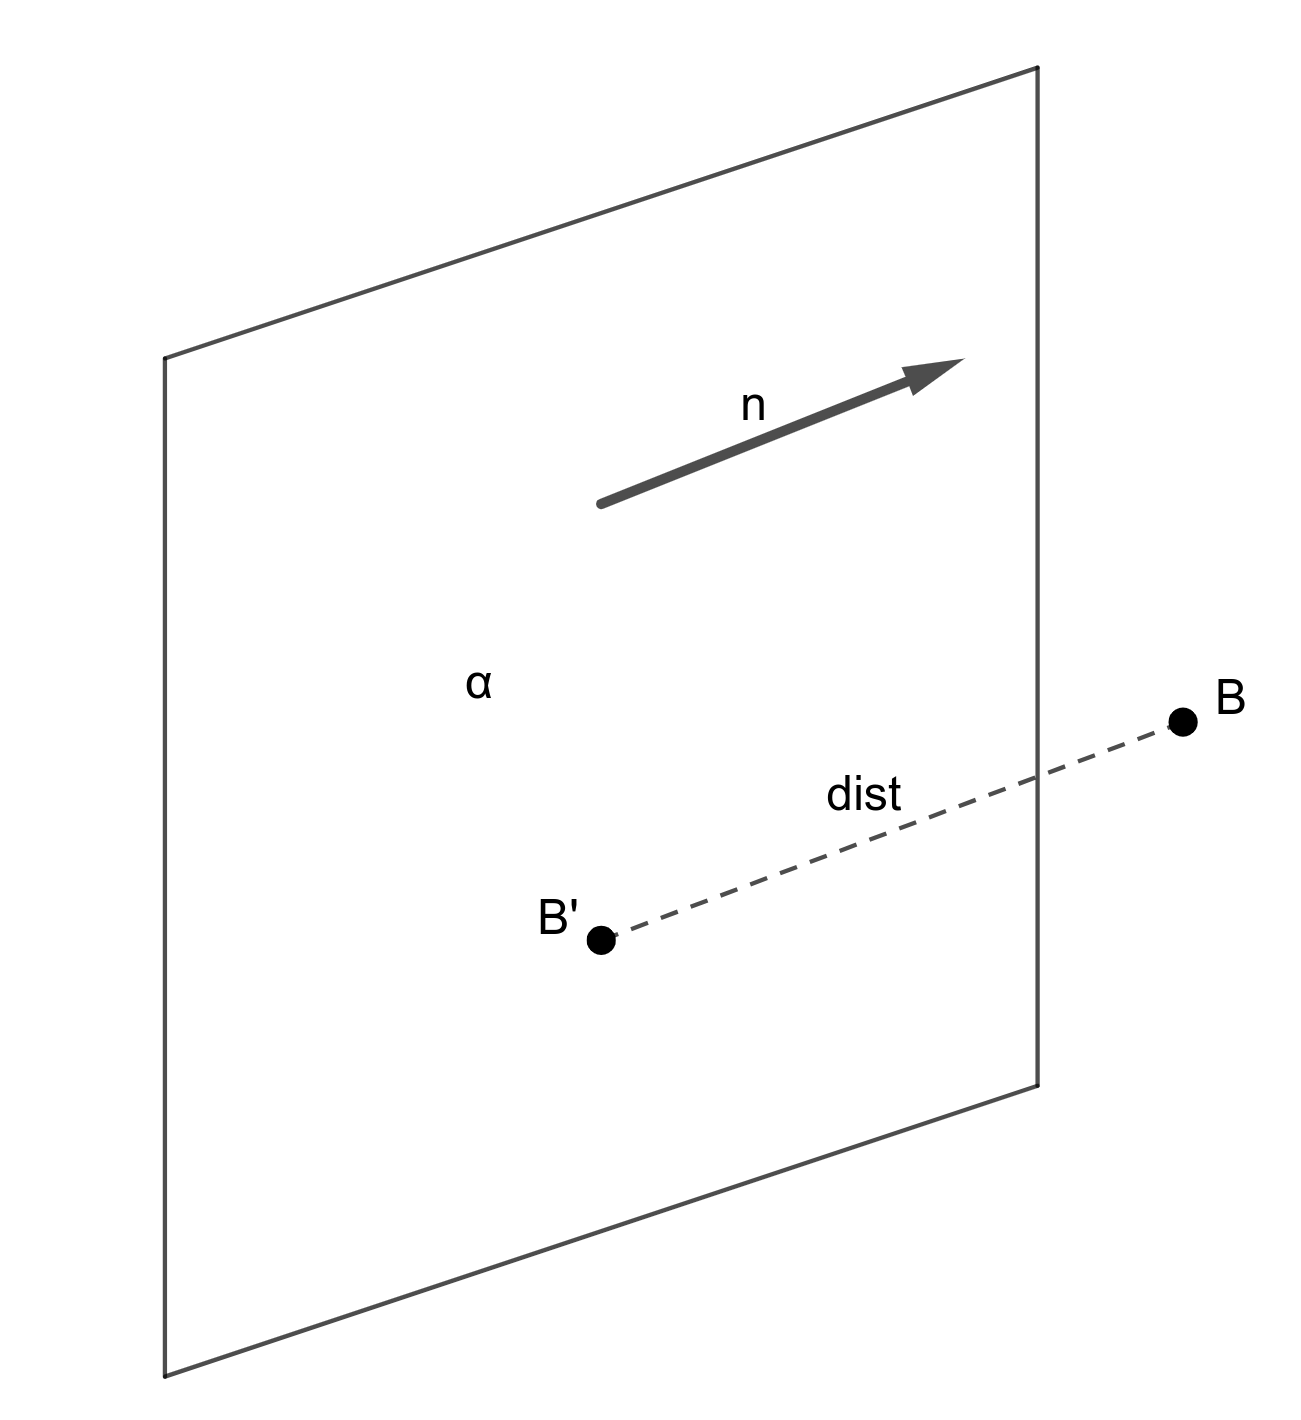
\includegraphics[width=7cm, scale=0.8]{ej-18/18ini.png}

	\noindent Ecuación del plano $\alpha$ dado: \\
	\indent $\alpha) \ \ 3x + 2y -5z = 0$

	\noindent Punto $B$ dado: \\
	\indent $B(2, 1, -1)$

	\noindent Vector $\overrightarrow{OB} = \vec{b}$: \\
	\indent $\vec{b} = (2, 1, -1)$

	\noindent Vector normal del plano: \\
	\indent $\vec{n}=(3, 2, -5)$

	\noindent Ecuaciones paramétricas de una recta ortogonal al plano $\alpha$: \textit{(solo con fines ilustrativos)}

	$r) \ \begin{cases}
			x = 2 + 3t \\
			y = 1 + 2t \\
			z = -1 - 5t
		\end{cases}$
\end{multicols}

\noindent Lo anterior nos presenta la siguiente situación:

\begin{center}
	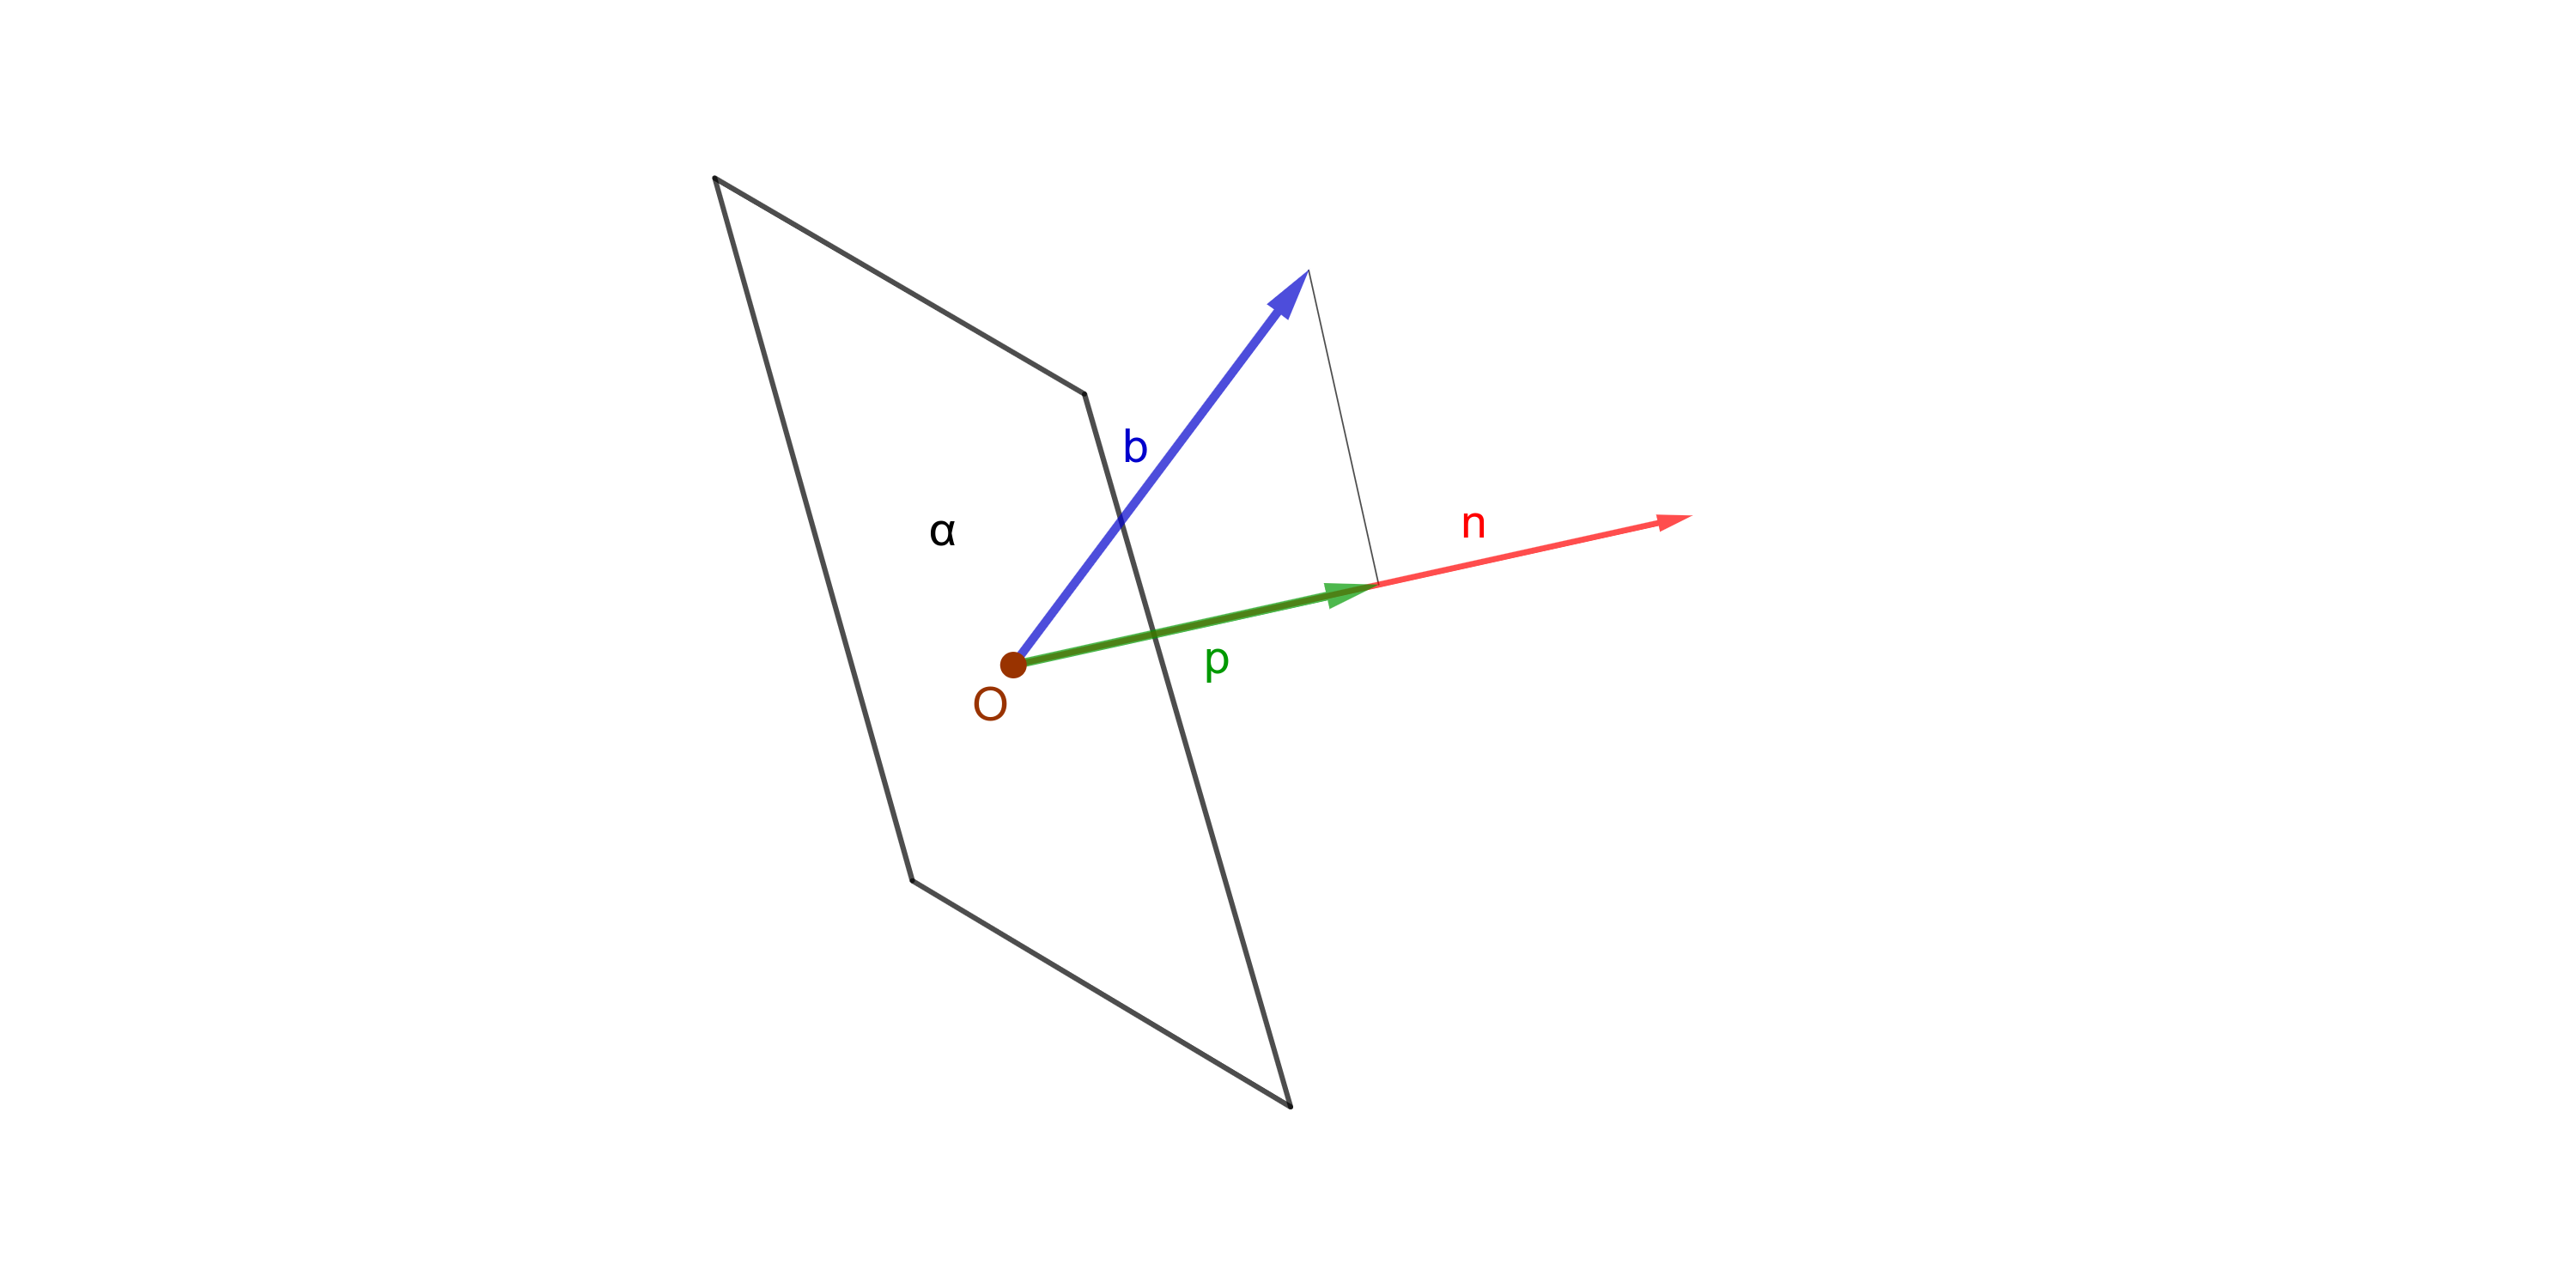
\includegraphics[width=10cm, scale=0.8]{ej-18/18ini2.png}
\end{center}

Ya que el coeficiente $d$ de $\alpha$ es igual a $0$, determinamos que el plano cruza el origen de coordenadas. El vector $\vec{n}$ representa el vector normal $\perp$ a $\alpha$, el vector $\vec{b}$ que representa la distancia $\overline{OB}$, con lo que la distancia del punto $B$ al plano $\alpha$ está determinada por el módulo del vector $\vec{p}$ \textit{(proyección de $\vec{b}$ sobre $\vec{n}$)}, que está dado por:

\begin{center}
	$\boxed{\overrightarrow{Proy_{\vec{n}} \ \vec{b}} = \cfrac{\vec{b} \cdot \vec{n}}{|\vec{n}|^2} \cdot \vec{n} = \vec{p}}$
\end{center}





% 2.2.1. Distancia de B a \alpha:
\newpage
\subsubsection{\texorpdfstring{Distancia del punto $B$ al plano $\alpha$:}{}}
\noindent Con la situación y los valores iniciales anteriormente mencionados procedemos a hallar la distancia del punto $B$ al plano $\alpha$, para ello hallamos el módulo de la proyección $\vec{p}$:
\begin{center}
	$|\vec{p}|  =\cfrac{|\vec{b} \cdot \vec{n}|}{|\vec{n}|} \hspace*{1cm} \vec{b}=(2, 1, -1) \hspace*{1cm} \vec{n}=(3, 2, -5)$
\end{center}
\begin{multicols}{2}
	\noindent Hallamos el producto escalar entre $\vec{b} \cdot \vec{n}$:
	\begin{align*}
		\vec{b} \cdot \vec{n} & = (2) \cdot (3) + (1) \cdot (2) + (-1) \cdot (-5) \\
		\vec{b} \cdot \vec{n} & = 6 + 2 + 5                                       \\
		\vec{b} \cdot \vec{n} & = \boxed{13}
		\columnbreak
	\end{align*}
	\noindent Hallamos el módulo de $\vec{n}$:
	\begin{align*}
		|\vec{n}| & = \sqrt{(3)^2 + (2)^2 + (-5)^2} \\
		|\vec{n}| & = \sqrt{9 + 4 + 25}             \\
		|\vec{n}| & = \boxed{\sqrt{38}}
	\end{align*}
\end{multicols}
\noindent Hallamos el módulo de la proyección de $\vec{b}$ sobre $\vec{n}$:

$|\vec{p}| =\cfrac{13}{\sqrt{38}} \implies \cfrac{13}{38}\sqrt{38}$

\noindent $\therefore$ \ La distancia del punto $B$ al plano $\alpha$ es \ \fcolorbox{black}{yellow}{$\cfrac{13}{38}\sqrt{38}$}  $\approx 2,109$

% 2.2.2. Coordenadas de B':
\newpage
\subsubsection{\texorpdfstring{Coordenadas del punto $B'$ que pertenece a $\alpha$ y cuya distancia a $B$ es igual que la distancia de $B$ a $\alpha$:}{}}
\noindent Para hallar el punto $B' \in \alpha$ y cuya distancia a $B$ es igual a la distancia de $B$ a $\alpha$ podemos hacer uso del vector proyección $\vec{p}$ antes mencionado para luego restarlo del vector $\vec{b}$, lo que nos da como resultado un vector $\vec{b'}$ cuyo sentido (punta flecha) coincidirá con el punto $B' \in \alpha$:
\begin{center}
	$\boxed{\vec{p} = \cfrac{\vec{b} \cdot \vec{n}}{|\vec{n}|^2} \cdot \vec{n}} \hspace*{1cm}
		\vec{n}=(3, 2, -5)  \hspace*{1cm}
		\vec{b}=(2, 1, -1) \hspace*{1cm}
		\vec{b} \cdot \vec{n}  = 13 \hspace*{1cm}
		|\vec{n}|  = \sqrt{38}$
\end{center}
\begin{multicols}{2}
	\noindent Calculamos $\vec{p}$:
	\begin{align*}
		\vec{p} & = \cfrac{\vec{b} \cdot \vec{n}}{|\vec{n}|^2} \cdot \vec{n}       \\
		\vec{p} & = \cfrac{13}{(\sqrt{38})^2} \cdot (3, 2, -5)                     \\
		\vec{p} & = \cfrac{13}{38} \cdot (3, 2, -5)                                \\
		\vec{p} & = \left( \cfrac{39}{38}, \cfrac{26}{38}, -\cfrac{65}{38} \right) \\
	\end{align*}
	\noindent Calculamos $\vec{b'}$:
	\begin{align*}
		\vec{b'} & = \vec{b} - \vec{p}                                                           \\
		\vec{b'} & = (2, 1, -1) - \left( \cfrac{39}{38}, \cfrac{26}{38}, -\cfrac{65}{38} \right) \\
		\vec{b'} & = \left( 2 - \cfrac{39}{38}, 1 - \cfrac{26}{38}, -1 + \cfrac{65}{38} \right)  \\
		\vec{b'} & = \left( \cfrac{37}{38}, \cfrac{12}{38}, \cfrac{27}{38} \right)
	\end{align*}
\end{multicols}

\noindent $\therefore$ \ Las coordenadas del punto $B'$ que está contenido en $\alpha$ y cuya distancia a $B$ es igual a la distancia de $B$ a $\alpha$ es:

\fcolorbox{black}{yellow}{$B'\left( \cfrac{37}{38}, \cfrac{12}{38}, \cfrac{27}{38} \right)$}
\ $\approx \ (0.974; \ 0.316;\ 0.711)$

\newpage
\noindent \textbf{Gráfica 18-a,b}:
\begin{center}
	\href{https://www.geogebra.org/3d/wrk3eabw}{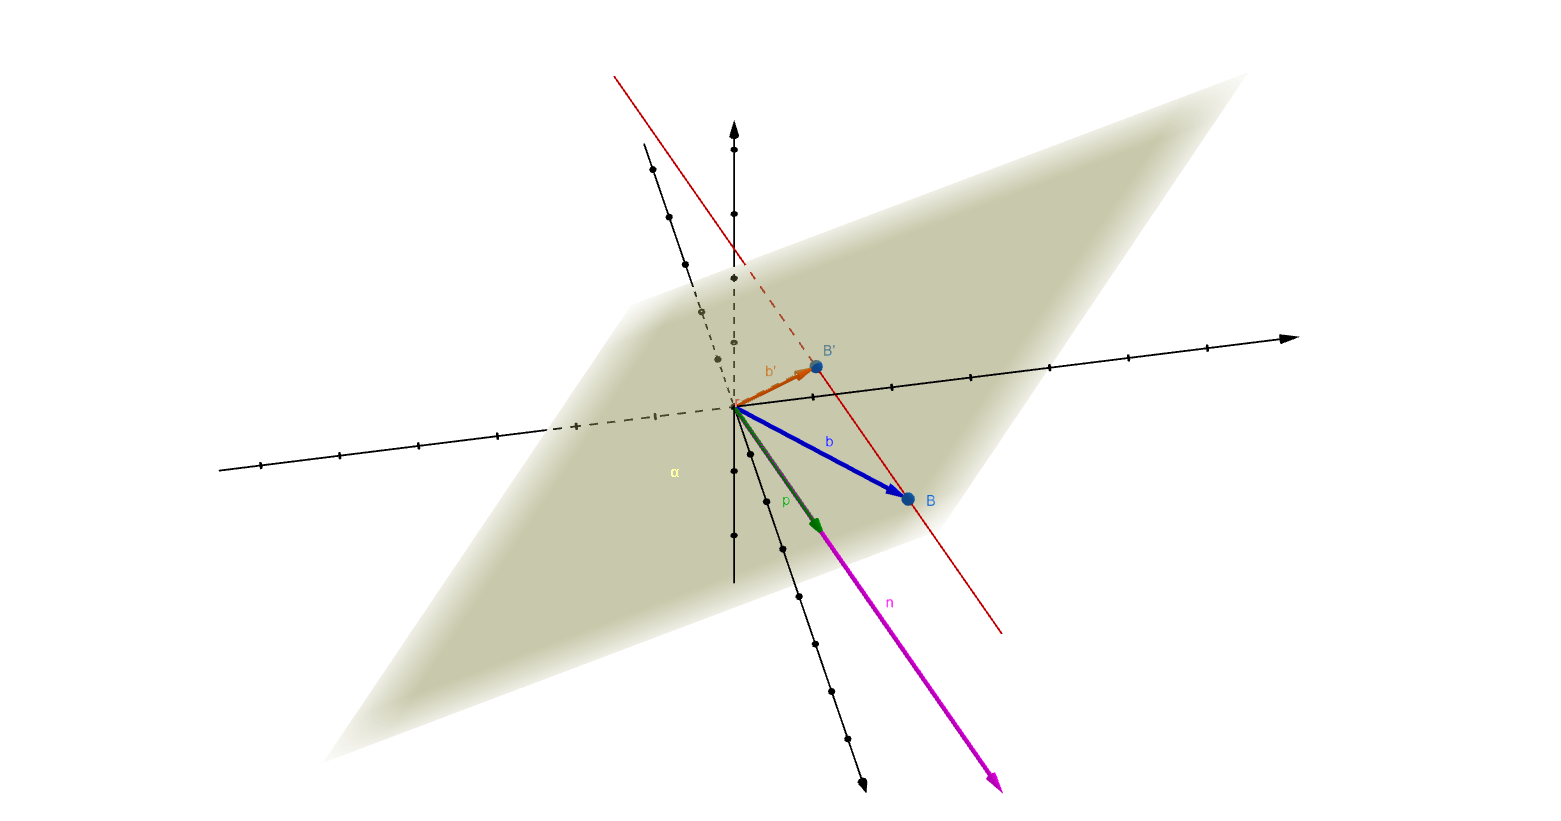
\includegraphics[width=15cm, scale=1]{TP-MATEMATICA-EJ18AB.png}}
\end{center}



